\documentclass[11pt]{report}

% Paquetes y configuraciones adicionales
\usepackage{graphicx}
\usepackage[export]{adjustbox}
\usepackage{caption}
\usepackage{float}
\usepackage{titlesec}
\usepackage{geometry}
\usepackage[hidelinks]{hyperref}
\usepackage{titling}
\usepackage{titlesec}
\usepackage{parskip}
\usepackage{wasysym}
\usepackage{tikzsymbols}
\usepackage{fancyvrb}
\usepackage{xurl}
\usepackage{subcaption}
% \usepackage{amsmath} 
\usepackage{listings}
\usepackage{xcolor}
\usepackage[spanish]{babel}
\usepackage{bookmark}

\newcommand{\subtitle}[1]{
  \posttitle{
    \par\end{center}
    \begin{center}\large#1\end{center}
    \vskip0.5em}
}

% Configura los márgenes
\geometry{
  left=2cm,   % Ajusta este valor al margen izquierdo deseado
  right=2cm,  % Ajusta este valor al margen derecho deseado
  top=3cm,
  bottom=3cm,
}

% Configuración de los títulos de las secciones
\titlespacing{\section}{0pt}{\parskip}{\parskip}
\titlespacing{\subsection}{0pt}{\parskip}{\parskip}
\titlespacing{\subsubsection}{0pt}{\parskip}{\parskip}

% Redefinir el formato de los capítulos y añadir un punto después del número
\makeatletter
\renewcommand{\@makechapterhead}[1]{%
  \vspace*{0\p@} % Ajusta este valor para el espaciado deseado antes del título del capítulo
  {\parindent \z@ \raggedright \normalfont
    \ifnum \c@secnumdepth >\m@ne
        \huge\bfseries \thechapter.\ % Añade un punto después del número
    \fi
    \interlinepenalty\@M
    #1\par\nobreak
    \vspace{10pt} % Ajusta este valor para el espacio deseado después del título del capítulo
  }}
\makeatother

% Configura para que cada \chapter no comience en una pagina nueva
\makeatletter
\renewcommand\chapter{\@startsection{chapter}{0}{\z@}%
    {-3.5ex \@plus -1ex \@minus -.2ex}%
    {2.3ex \@plus.2ex}%
    {\normalfont\Large\bfseries}}
\makeatother

% Define los colores que deseas usar para resaltar código
\definecolor{codegreen}{rgb}{0,0.6,0}
\definecolor{codegray}{rgb}{0.5,0.5,0.5}
\definecolor{codepurple}{rgb}{0.58,0,0.82}
\definecolor{backcolour}{rgb}{0.95,0.95,0.92}

% Configuración de estilo para el código
\lstdefinestyle{mystyle}{
    backgroundcolor=\color{backcolour},   
    commentstyle=\color{codegreen},
    keywordstyle=\color{magenta},
    numberstyle=\tiny\color{codegray},
    stringstyle=\color{codepurple},
    basicstyle=\ttfamily\footnotesize,
    breakatwhitespace=false,         
    breaklines=true,                 
    captionpos=b,                    
    keepspaces=true,                 
    numbers=left,                    
    numbersep=5pt,                  
    showspaces=false,                
    showstringspaces=false,
    showtabs=false,                  
    tabsize=2
}

\begin{document}

% Portada del informe
\title{Estudio de la influencia de la arquitectura y de la organización interna en el rendimiento}
\subtitle{Diseño de Procesadores}
\author{Carlos Pérez Fino \texttt{alu0101340333@ull.edu.es} \and Cheuk Kelly Ng Pante \texttt{alu0101364544@ull.edu.es}}
\date{\today}

\maketitle

\pagestyle{empty} % Desactiva la numeración de página para el índice

% Índice
\tableofcontents

% Nueva página
\cleardoublepage

\pagestyle{plain} % Vuelve a activar la numeración de página
\setcounter{page}{1} % Reinicia el contador de página a 1

% Secciones del informe
% Capitulo 1
\chapter{Introducción}
The aim of this project is to address the hardware implementation of a processor, in this case the Nios II, which optimises performance in solving a specific problem, in this case that of applying a convolution filter on an original image.
in the resolution of a specific problem, in this case that of applying a convolution filter on an original image.

To start the project, a previous activity was the tutorial on the development of Nios II, and once the tutorial was finished, we proceeded to the realisation of the project. 
tutorial was completed, some test programs were created in order to familiarise ourselves with the development environment and with the
Nios II processor. After testing that the development environment and the processor work correctly, we proceeded to improve the design by measuring the performance of each improvement.
by measuring the performance of each improvement. It was found that introducing different types of memory took about the same amount of time for the different enhancements.
for the different improvements. To check the times, the following program was run:

\lstset{style=mystyle}
\lstinputlisting[language=C]{./code/test_memories.c}

% Capitulo 2
\chapter{Desarrollo del filtro de convolución, filtro Gaussiano}
Para el desarrollo del filtro de convolución se ha utilizado el filtro Gaussiano. El filtro Gaussiano es un filtro que se utiliza para
suavizar una imagen. Se ha utilizado este filtro porque es un filtro que se utiliza mucho en el procesamiento de imágenes y es un filtro
que se puede aplicar a cualquier imagen. El filtro Gaussiano se aplica a una imagen para suavizarla y eliminar el ruido de la imagen.

\section{Implementación del filtro Gaussiano}
Para la implementación del filtro Gaussiano se ha utilizado el siguiente código:
\lstset{style=mystyle}
\lstinputlisting[language=C]{./code/gaussian_filter.c}

Este algoritmo se ha implementado en C y lo primero lo que se hace es definir el kernel del filtro Gaussiano. El kernel del filtro
Gaussiano es una matriz de 3x3 que se utiliza para aplicar el filtro a la imagen. Tiene la siguiente forma:

\begin{center}
  $\left[
  \begin{array}{ccc}
    1 & 2 & 1 \\
    2 & 4 & 2 \\
    1 & 2 & 1 \\
  \end{array}
  \right]$
\end{center}

Este kernel se utiliza para aplicar el filtro Gaussiano a la imagen. Para aplicar el filtro Gaussiano a la imagen se recorre la imagen
y se aplica el filtro a cada píxel de la imagen. Para aplicar el filtro a un píxel se recorre la matriz del kernel y se multiplica cada
elemento de la matriz por el píxel de la imagen correspondiente. Una vez se han multiplicado todos los elementos de la matriz del kernel
por el píxel de la imagen se suman todos los resultados y se divide entre 16. El resultado de esta operación es el nuevo valor del píxel
de la imagen que se está procesando.

% La imagen original es de 512x512 y devuelve una imagen de 510x510
La función \texttt{gaussian\_filter} recibe como parámetros la imagen de entrada y la imagen de salida. La imagen de entrada es la imagen
original que se quiere suavizar y la imagen de salida es la imagen suavizada. Esta función lee la imagen de entrada y crea una imagen de con 
la función \texttt{pgmread2}. Una vez se ha leído la imagen de entrada lo que se hace es reservar memoria para la imagen de salida, que tendrá
dimensiones (row - 2) x (col - 2) debido al borde que no se puede procesar completamente. Luego, reserva memoria para cada fila de la imagen
de salida. A continuación, se hace la convolución de la imagen con el kernel del filtro Gaussiano. Para ello, recorre cada pixel excluyendo los 
bordes de la imagen, excluyendo los bordes de (1 a row - 1) y (1 a col - 1). Para cada pixel en la posición (i, j), calcula la suma de la
multiplicación de cada pixel de la imagen con el kernel del filtro Gaussiano. Finalmente, divide la suma entre 16 y guarda el resultado en la
imagen de salida 'output'. 

A continuación, se escribe la imagen de salida en un archivo con la función \texttt{pgmwrite2}. Esta función es la encargada de escribir la imagen
en un archivo con el formato PGM y se le pasa como parámetros el nombre del archivo, las dimensiones de la imagen y la imagen en sí. Finalmente,
se libera la memoria de la imagen de entrada y de la imagen de salida.

\newpage

\chapter{Estudios y resultados}
A la hora de realizar el estudio, se ha optado por hacer cinco pruebas diferentes para poder comparar los resultados y ver cuál es la mejor
opción para mejorar el rendimiento del procesador. Para hacer las pruebas los tiempos se han obtenido haciendo un promedio de 5 ejecuciones
de cada prueba. Las pruebas que se han realizado son las siguientes:

\begin{table}[H]
  \centering
  \begin{tabular}{|c|c|}
    \hline
    \textbf{Prueba} & \textbf{Tiempo obtenido en segundos} \\ \hline
    Sin cambios & 18.96 \\ \hline
    CPU con mayores prestaciones (Nios II/f) & 18.98 \\ \hline
    Hardware divide & 18.92 \\ \hline
    Nios II/f y Hardware divide & 18.97 \\ \hline
    Caché para datos & 18.90 \\ \hline
  \end{tabular}
\end{table}

\section{CPU con mayores prestaciones}
Analizando los resultados obtenidos, al cambiar la CPU a uno con mayores prestaciones (Nios II/f) no obtenemos mucha diferencia pero observamos
que tarda un poquillo más, por algún motivo que desconocemos. En cambio, en la ejecución del programa si es verdad que la diferencia es casi 
imperceptible pero si mejor algo.

\begin{figure}[H]
  \centering
  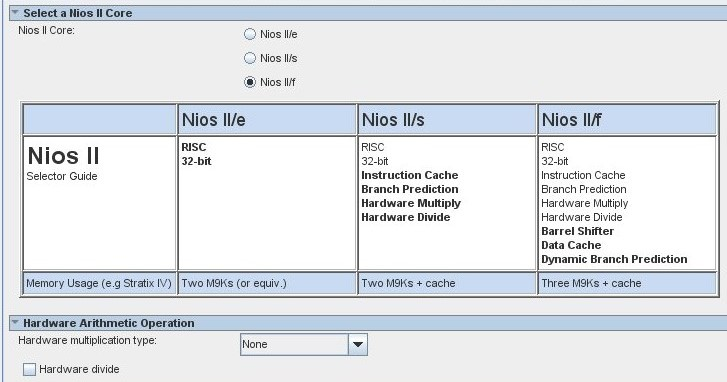
\includegraphics[scale=0.8]{img/cpu_mayores_prestaciones.jpeg}
  \caption{Configuración de la CPU con mayores prestaciones}
\end{figure}

\newpage

\section{Hardware para multiplicación y división}
En la siguiente prueba se ha añadido hardware para la multiplicación y la división. En esta prueba se ha obtenido un tiempo de 18.92 segundos,
lo que supone una mejora de 0.04 segundos respecto a la prueba anterior. Aunque la mejora no es muy significativa, se puede observar que el
hardware para la multiplicación y la división ha mejorado el rendimiento del procesador.

\begin{figure}[H]
  \centering
  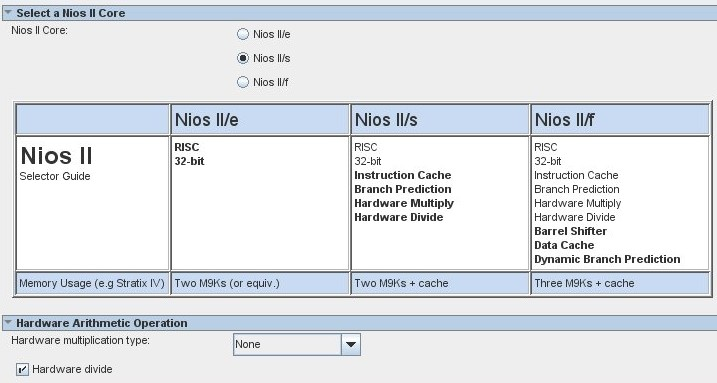
\includegraphics[scale=0.8]{img/activo_hardware_divide.jpeg}
  \caption{Configuración del hardware para la multiplicación y la división}
\end{figure}

\newpage

\section{CPU con mayores prestaciones y hardware para multiplicación y división}
En la siguiente prueba se han combinado las dos mejoras anteriores, es decir, se ha cambiado la CPU a una con mayores prestaciones y se ha añadido
hardware para la multiplicación y la división. En esta prueba ha supuesto un empeoramiento respecto a la prueba original. No sabemos por qué
ha ocurrido esto, pero se puede deber a que la CPU con mayores prestaciones no es compatible con el hardware para la multiplicación y la división.

\begin{figure}[H]
  \centering
  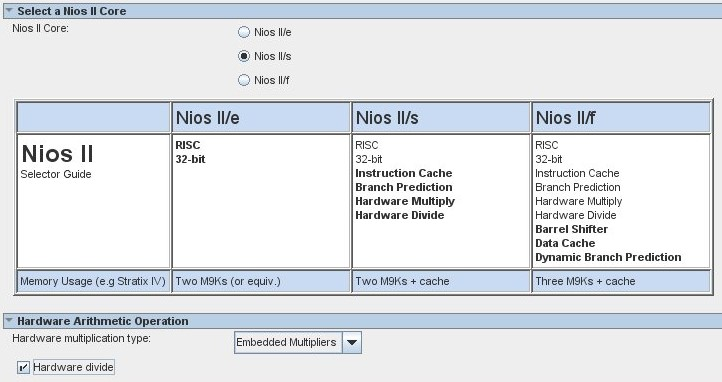
\includegraphics[scale=0.8]{img/hardware_multiplicacion_division.jpeg}
  \caption{Configuración de la CPU con mayores prestaciones y hardware para la multiplicación y la división}
\end{figure}

\newpage

\section{Caché para datos}
En la última prueba se ha añadido una caché de instrucciones de datos. En esta prueba se ha obtenido un tiempo de 18.90 segundos, lo que supone
una mejora de 0.06 segundos respecto a la prueba original. Aunque la mejora no es muy significativa, se puede observar que la caché de instrucciones
de datos ha mejorado el rendimiento del procesador. 

Primero se ha asignado el tamaño de la caché de datos, llevando a un conflicto con la memoria onchip. Para solucionar este problema, se redujo
el tamaño de la memoria onchip pasando de los 20KB a 10KB.

Haciendo esto permitía crear una caché de unos 8KB, lo cual tuvo un impacto positivo en el rendimiento del procesador y se redujo un poco el tiempo
de ejecución.

\begin{figure}[H]
  \centering
  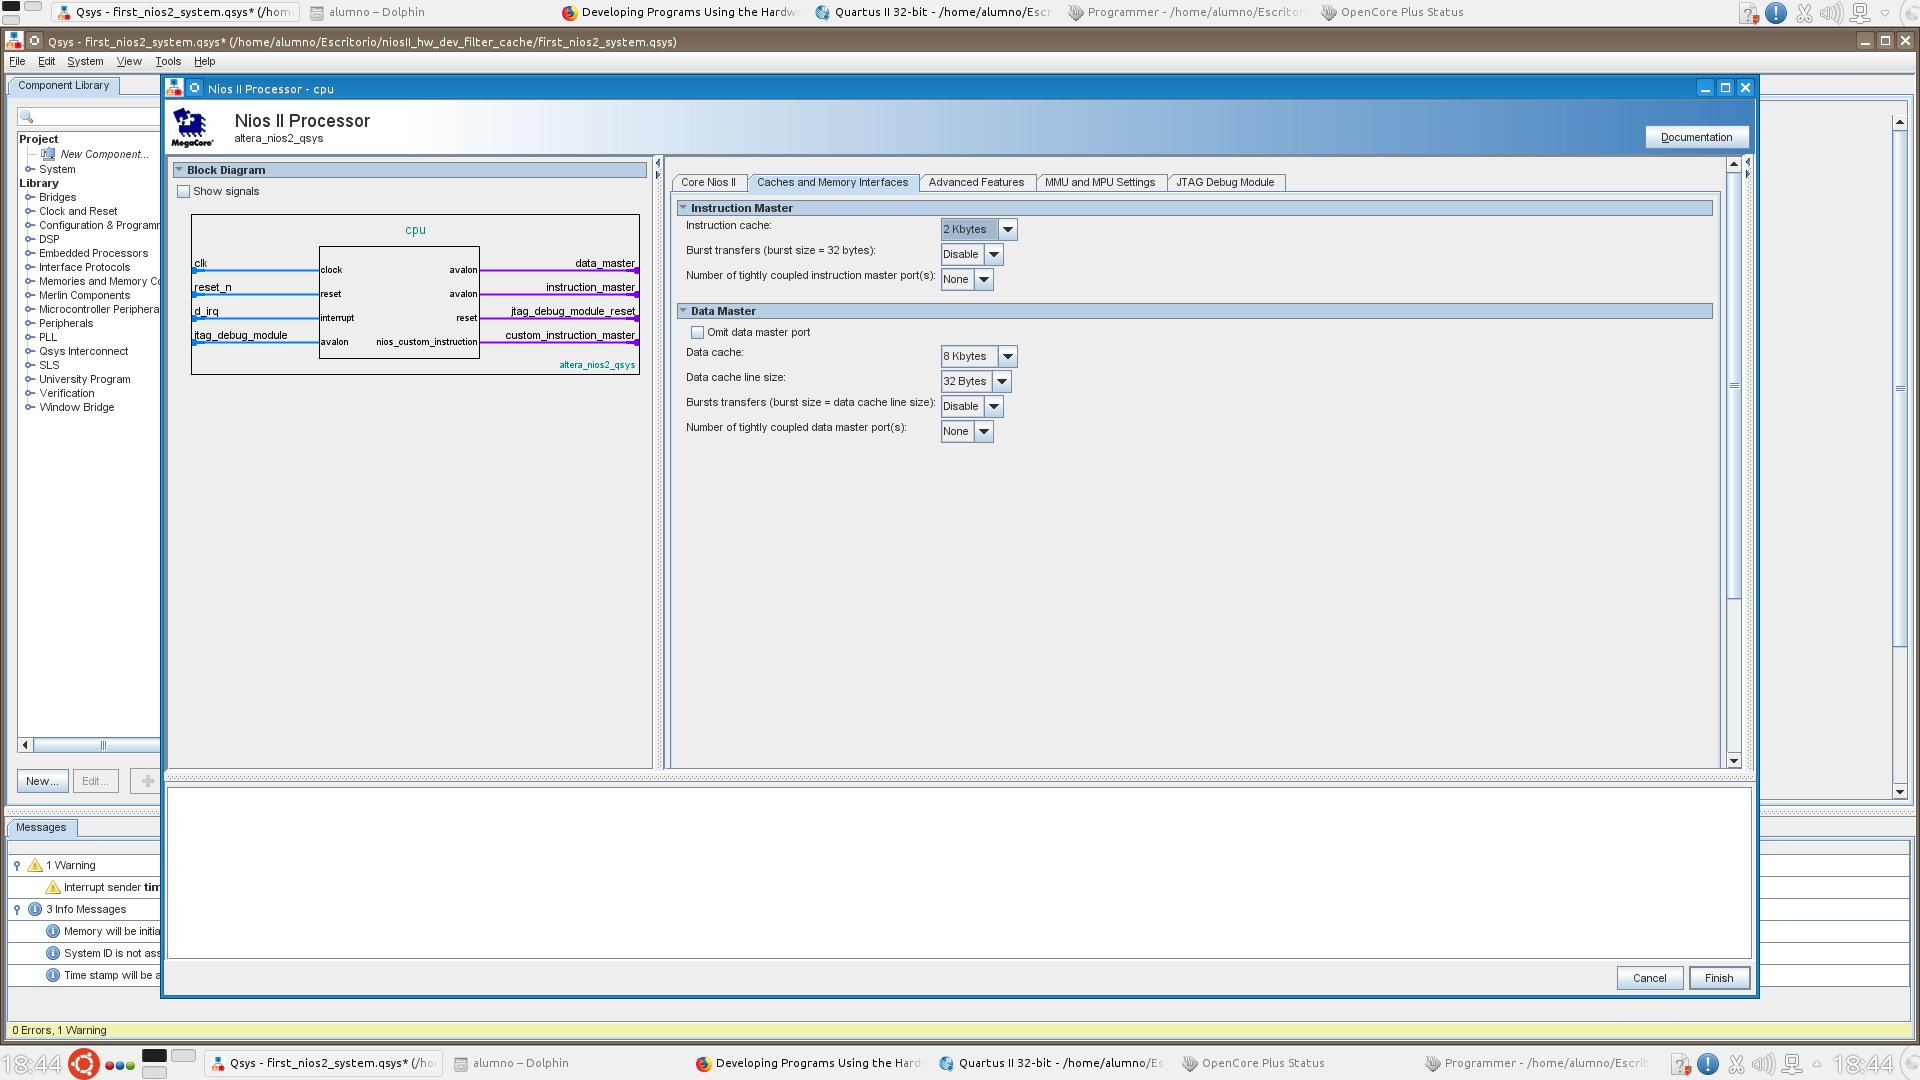
\includegraphics[scale=0.34]{img/cache_8KB.jpeg}
  \caption{Configuración de la caché de datos}
\end{figure}

\newpage

\chapter{Tightly coupled memory}
Como útlima mejora se ha añadido una memoria tightly coupled memory. La tightly coupled memory es una memoria que se conecta directamente al
procesador y se utiliza para almacenar datos que se utilizan con frecuencia. 

\begin{figure}[H]
  \centering
  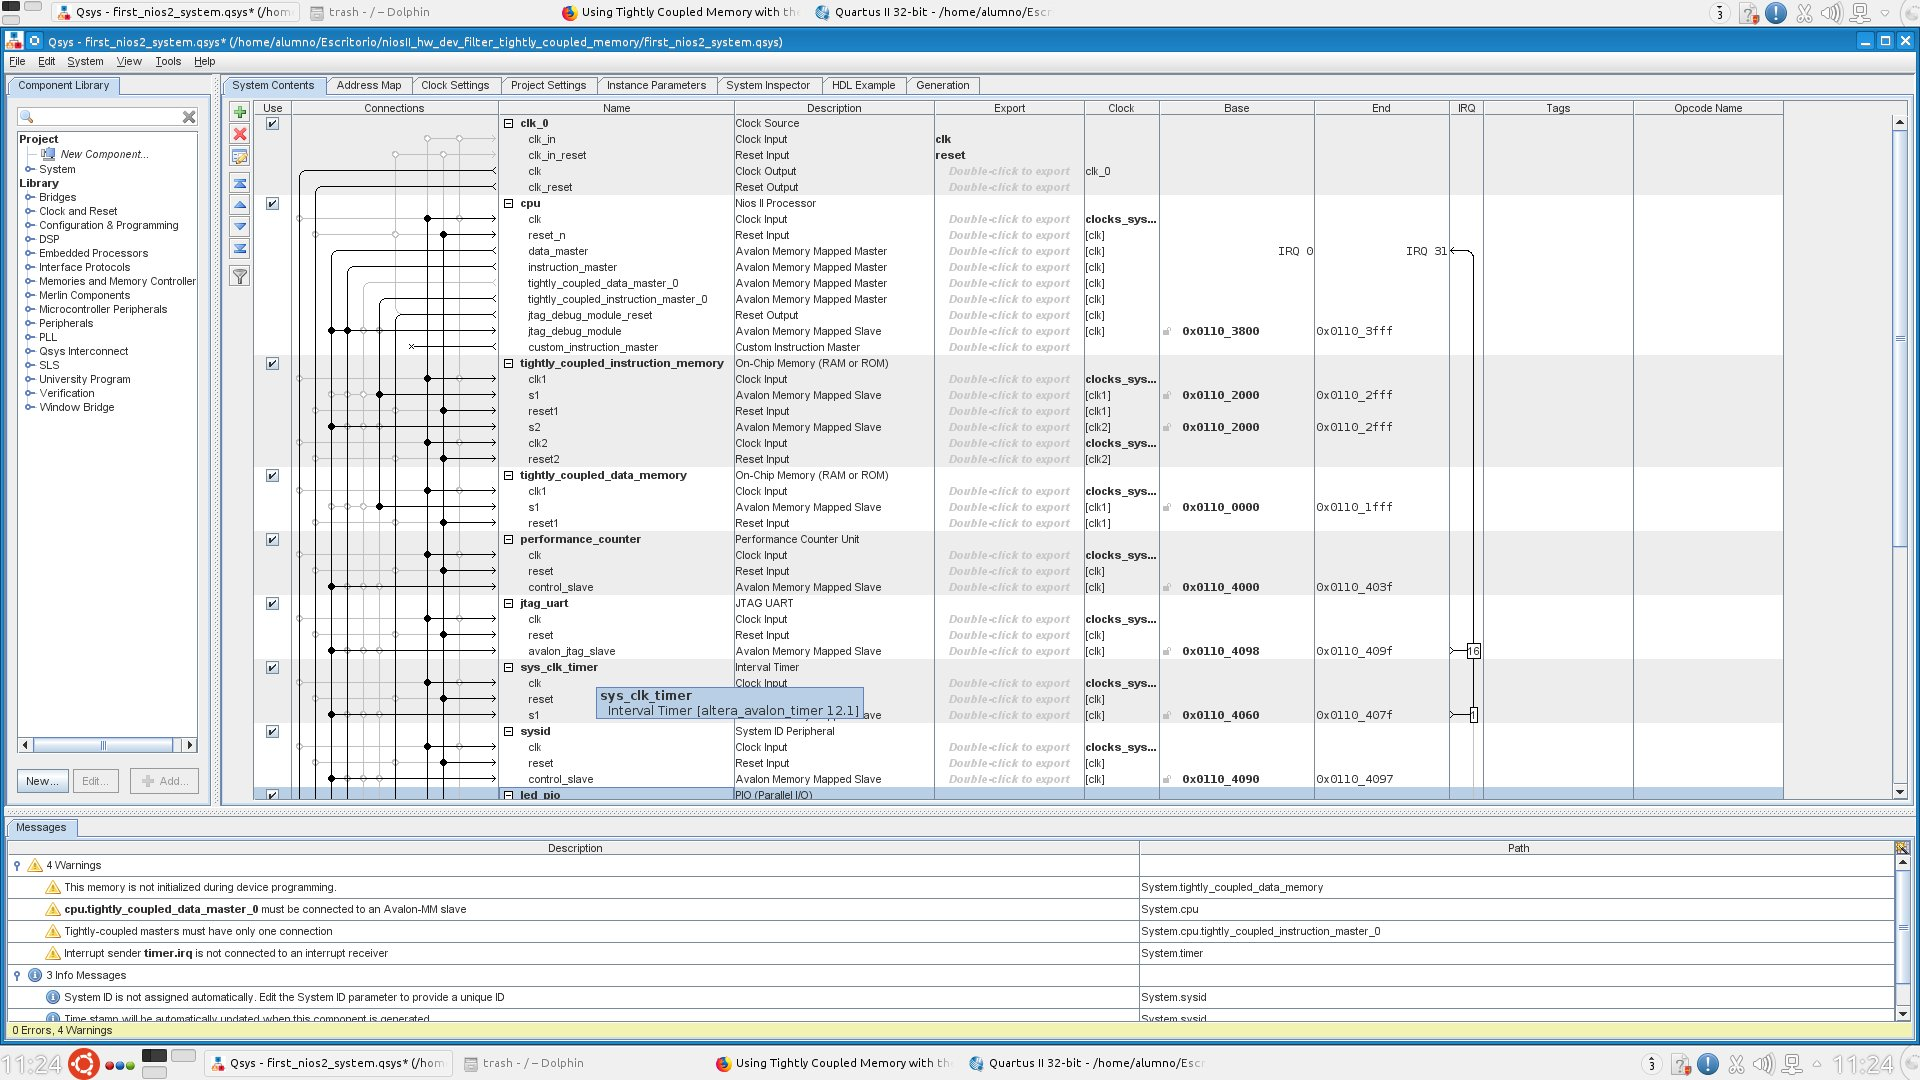
\includegraphics[scale=0.34]{img/tightly_coupled_memory.jpeg}
  \caption{Configuración de la tightly coupled memory}
\end{figure}

Se ha añadido los módulos de memoria habría que programar el modelo y hacer la mediciones de tiempo para ver si ha mejorado el rendimiento del
procesador. No obstante, no se ha podido realizar esta mejora debido a problemas con la implementación de la tightly coupled memory. Se ha seguido
el tutorial de Altera para la implementacion de esta memoria pero no se ha podido realizar correctamente. Uno de los problemas era abrir la terminal
de Nios II y localizar donde se encontraba.

\newpage

\chapter{Conclusiones}
En este proyecto ha servido para aprender a utilizar el procesador Nios II y a mejorar su rendimiento. Se ha realizado un estudio para ver cómo
mejorar el rendimiento del procesador y se han realizado varias pruebas para comparar los resultados. Se ha observado que la caché de instrucciones
de datos ha mejorado el rendimiento del procesador y se ha obtenido una mejora de 0.06 segundos en el tiempo de ejecución.

Por otro lado a la hora de realizar las mediciones, los resultados no eran los esperados por el resultado dado del \texttt{clock()} ya que al realizar 5 repeticiones
para aplicar el filtro estabamos aproximadamente 12 minutos esperando a que se ejecutara el programa y luego poniamos temporizadores al inicio final de la ejecucion del
programa y daba tiempos de 25 segundos aproximadamente. Por lo que no se ha podido realizar correctamente las mediciones de tiempo pero se ha podido observar
que con algunas mejoras se ha podido mejorar el rendimiento del procesador.

Además, otros problemas que se han encontrado a lo largo del proyecto han sido con el propio Quartus, al ser una version del programa bastante antiguo y
no tener mucha experiencia con el programa y con el poco soporte online, ha sido complicado realizar algunas tareas. También, había veces que se hacía
pequeños cambios en la configuración del proyecto BSP y saltaban errores que no se sabía por qué ocurrían y habia que empezar de nuevo. 

\end{document}